\documentclass{article}
\usepackage{graphicx}
\usepackage{url}
\usepackage{indentfirst}


\begin{document}

\title{Perception of surroundings:}
\maketitle

\section{Introduction}

The main goal of our project is to make the card system at the University of Porto more sustainable and practical, through a digital wallet that will allow students and staff at the University of Porto to use their card via a mobile phone.
Considering that our target audience will be the academic community of the University of Porto, we decided to create and share a survey in order to understand what would be the best approach to develop our application and
to obtain knowledge about users' expectations of our application, as well as their familiarity with technology and their priorities in a digital wallet.

\section{Analysis of responses}


We obtained a total of 48 responses, all from students currently enrolled at a Higher Education Institution. Considering the target audience previously defined, this indicates that all the responses will be valuable, as they represent possible users of the application.

\begin{figure}[h]
    \centering
    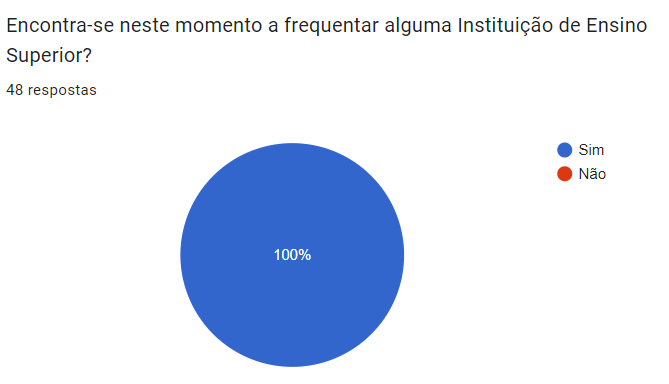
\includegraphics[width=0.7\textwidth]{images/questionaire1.png}
    \caption{Your caption}
\end{figure}


+
\subsection{Frequency and use cases}

Around 60\% of users responded that they used their institutional card frequently, with the most used services being: \textbf{Access to the canteen} (~64\%), \textbf{Access to classrooms/cores} (50\%) and \textbf{Identification in tests/exams} (~44\%).
This suggests that it will be crucial to create a quickly accessible application for occasional, short-term use, as well as the possibility of it serving as a means of institutional identification for the user holding the virtual card.

\begin{figure}[h]
    \centering
    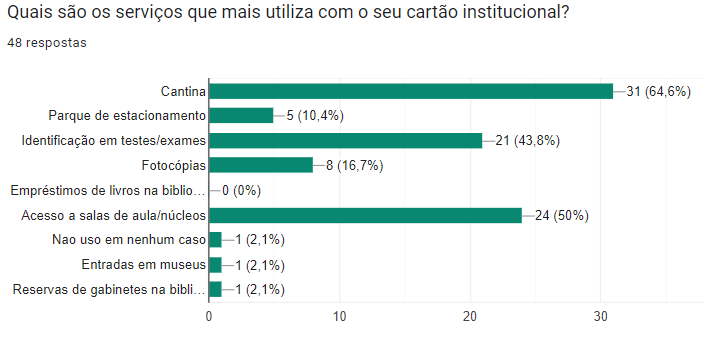
\includegraphics[width=0.9\textwidth]{images/questionaire2.png}
    \caption{Your caption}
\end{figure}

\begin{figure}[h]
    \centering
    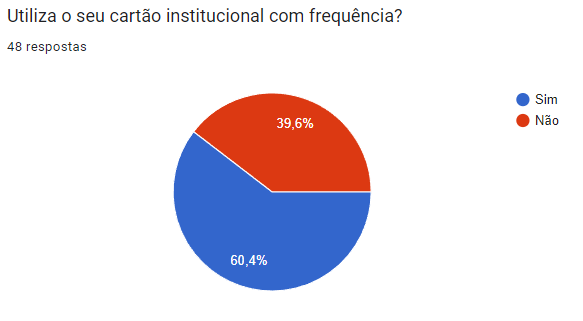
\includegraphics[width=0.9\textwidth]{images/questionaire3.png}
    \caption{Your caption}
\end{figure}

\subsection{Previous experience with technologies}

All but one of the participants answered that they had previous experience with virtual cards, and of the 47 relevant answers, 35 (75\%) reported a very good experience using it. We therefore concluded that our target audience felt comfortable with the technologies used, which will allow us to use current applications that implement these functionalities as inspiration.
Through the survey, we were also able to analyze some of the difficulties that some participants had using similar applications:
\begin{itemize}
    \item \textbf Virtual card creation process
    \item \textbf Errors in carrying out the different operations using the application.
\end{itemize}


These difficulties allow us to conclude that we must make these processes intuitive and provide support to users.



\subsection{Expectations and suggestions}

According to the expectations of potential future users, we see a greater interest in the security of the application (77\%) as well as the convenience it will bring (71\%). We therefore need to focus on guaranteeing the security of the users' data and the convenience of using the solution to justify the possible replacement of the physical card in many cases.
We also noticed an interest in a simple interface for the application (52\%).

\begin{figure}[h]
    \centering
    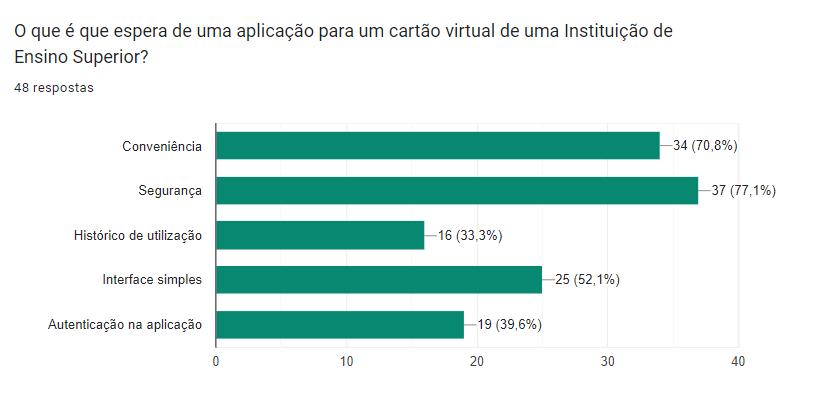
\includegraphics[width=1\textwidth]{images/questionaire4.png}
    \caption{Your caption}
\end{figure}

\end{document}
